We have shown that the spectrum of the emitted power by a THz antenna is influenced by several efficiency factors. Bandwidth is especially limited by RC roll-off and lifetime roll-off. We also discussed why only some antenna topologies are applicable in THz-TDS. In this thesis, only H-Dipole antennas and I-shaped dipole antennas are investigated. Both antenna types are fabricated with pads that are needed to read the photocurrent that is generated by the incident THz transient. The pads however influence the detected THz spectrum as will be shown in the following. 

\subsection{Fourier Transformation}


\begin{figure}[!]
    \centering
    \begin{minipage}{\textwidth} 
        \centering
        \begin{subfigure}[t]{0.48\textwidth}
            \centering
            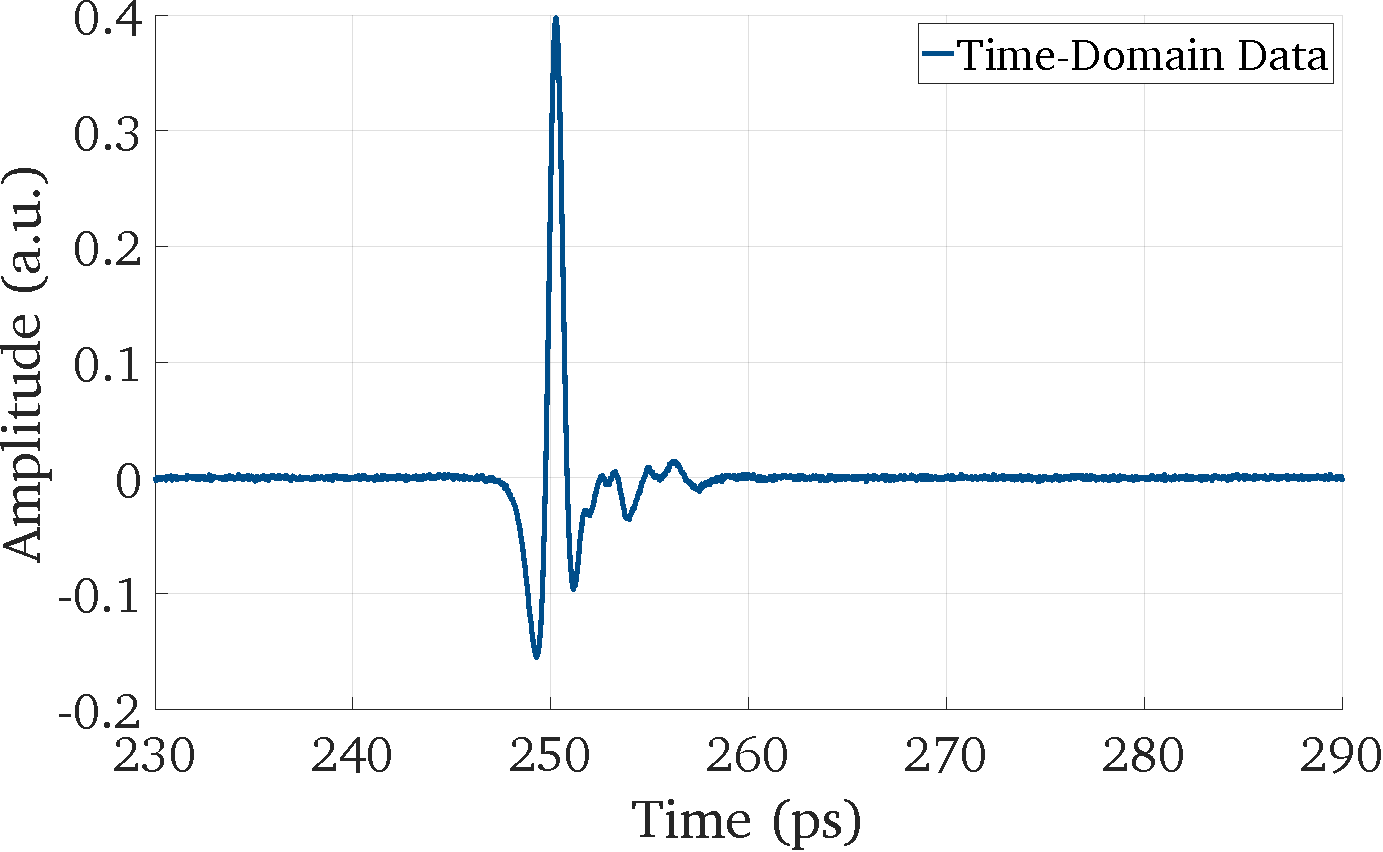
\includegraphics[height=0.235\textheight]{figures/theory/time_domain.pdf}
            \caption{\centering}
            \label{fgdhsjk}
        \end{subfigure}
        \hfill
        \begin{subfigure}[t]{0.48\textwidth}
            \centering
            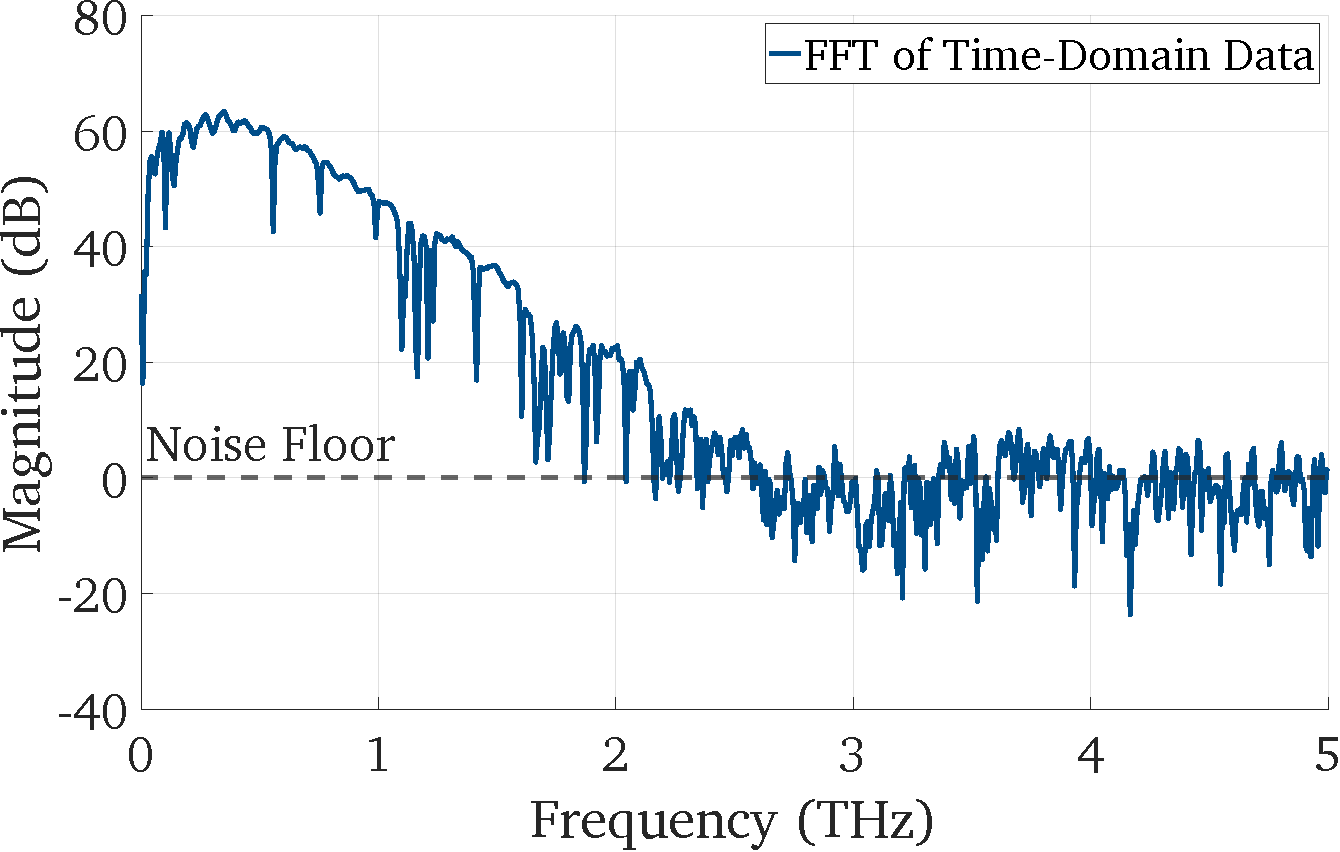
\includegraphics[height=0.235\textheight]{figures/theory/spectrum.pdf}
            \caption{\centering}
            \label{ghjkl}
        \end{subfigure}
        \caption{Exemplary FFT of a time-domain THz pulse. (a) Time-domain data. (b) FFT spectrum.}
        \label{fig:FFT}
    \end{minipage}
\end{figure}

As described previously, the emitted THz spectrum is obtained by Fourier transforming the measured time-domain THz signal. The Fourier transform of a real-valued time-domain pulse is a complex-valued frequency-domain spectrum. Analytically this yields \cite{MathematicalMethodsPhysics} 
\begin{equation}
    \mathcal{F}\left\{
        E_{Thz}(t) 
    \right\} = \beta \int_{-\infty}^{+\infty} E_{THz}(t)e^{i\omega t} = E_{THz}(\omega),
\end{equation}

where $\beta$ is a normalization factor that may differ depending on the field of study and the algorithm used. For discrete data, the analytical Fourier transform cannot be used. In this work, the fast Fourier transform (FFT) is used to obtain the THz spectrum. The FFT is an efficient implementation of the discrete Fourier transformation (DFT). The DFT maps a finite number of measurements $x(n)$ into the frequency domain. Many DFT properties are similar to the analog Fourier transformation. The DFT is defined as \cite{raoFastFourierTransform2010}
\begin{equation}
    X^F(k) = \beta \sum_{n = 0}^{N - 1}x(n)e^{\frac{-i2\pi k n}{N}}, \qquad k = 0, 1, ..., N-1, \qquad n = 0, 1, ..., N-1,
\end{equation}

where $x(n)$ denotes a uniformly sampled sequence and $X^F(k)$ is the $k$-th DFT coefficient. Figure \ref{fig:FFT} exemplary shows a THz trace in the time-domain and its Fourier transformation.

\subsection{Low Frequency Pad Resonances}
The pads used in the H-Dipole and I-shaped dipole antennas act as read-out terminals. A photocurrent is measured. The photocurrent is proportional to the incident THz radiation.  The pads are usually not part of the actual radiating element of the antenna. At low THz frequencies however, the pads influence the detected THz spectrum. At frequencies around \num{50} - \num{100} \si{\giga \hertz}, the wavelength of the THz radiation is considerably large at \num{3} - \num{6} \si{\milli \meter}. Electromagnetic waves couple most efficiently to resonant structures. Resonant in this context means a structure with a width that is a multiple of the EM-waves wavelength. Typically those multiples are $\frac{1}{4}$, $\frac{1}{2}$ or \num{1}. The PCAs electrodes are only a few micrometers wide. This results in the THz waves coupling to the antenna's pads rather than the electrodes at low frequencies. The large pads result in large surface currents which in turn result in a resonant behavior of the antenna at low frequencies. 

The low frequency resonances present a problem concerning the desired performance characteristics for PCAs used in pulsed systems. The measured time-domain trace of the THz radiation is dominated by low-frequency waves as they are much larger in amplitude. Since the resonances generate the strongest signals, the acquisition card in the read-out electronics becomes saturated. Most time, especially the higher THz frequencies are of interest. In cases where the measured signal is dominated by low frequency resonances, the higher frequency components can not be differentiated from noise as they are outweighed by the low frequency components when calculating the DFT. The high frequency limit of the PCA is thus not only limited by intrinsic roll-off factors and RC roll-off but also by the antenna topology, which is undesirable. Additionally, in some applications, a relatively flat antenna behavior given a specific frequency range is desired. Resonant spikes mean that an antenna's performance varies drastically for small changes in a signal's frequency that is to be detected.  In chapter 3, a solution to tackle the low frequency resonance problem is introduced.

\subsection{Low Frequency Time-Domain Harmonics}
Another unwanted effect at lower frequencies ($\nu < 500$ \si{\giga \hertz}) are resonant harmonics that are observable in the measured THz field. Reflections of non-radiative frequencies within the antenna's finite length feeding strip produce standing waves spaced apart by $\sim$\num{50} \si{\giga \hertz} with an effective wavelength equal to the strip's length. The resonant standing waves exhibit different propagation speeds compared to the emitted THz pulse. The dispersion causes undesired time-harmonic oscillations following the original THz pulse. Especially when investigating materials with high refractive indices, these time-harmonic oscillations can make measurements extremely challenging. Considering a very simplified case with normal incidence and where there is no distinction between the polarization of two materials, Fresnel's equations tell us that the reflectance $R$ becomes 
\begin{equation}
    R = \left| \frac{n_1 - n_2}{n_1 + n_2} \right|^2.
\end{equation}
A material with a high refractive index generally causes more reflections \cite{gallegosRefractiveIndex2025}. The actual THz signal may be hard to distinguish from the resonances caused by the standing wave propagation. 

\begin{figure}[ht]
  \centering
    \centering
    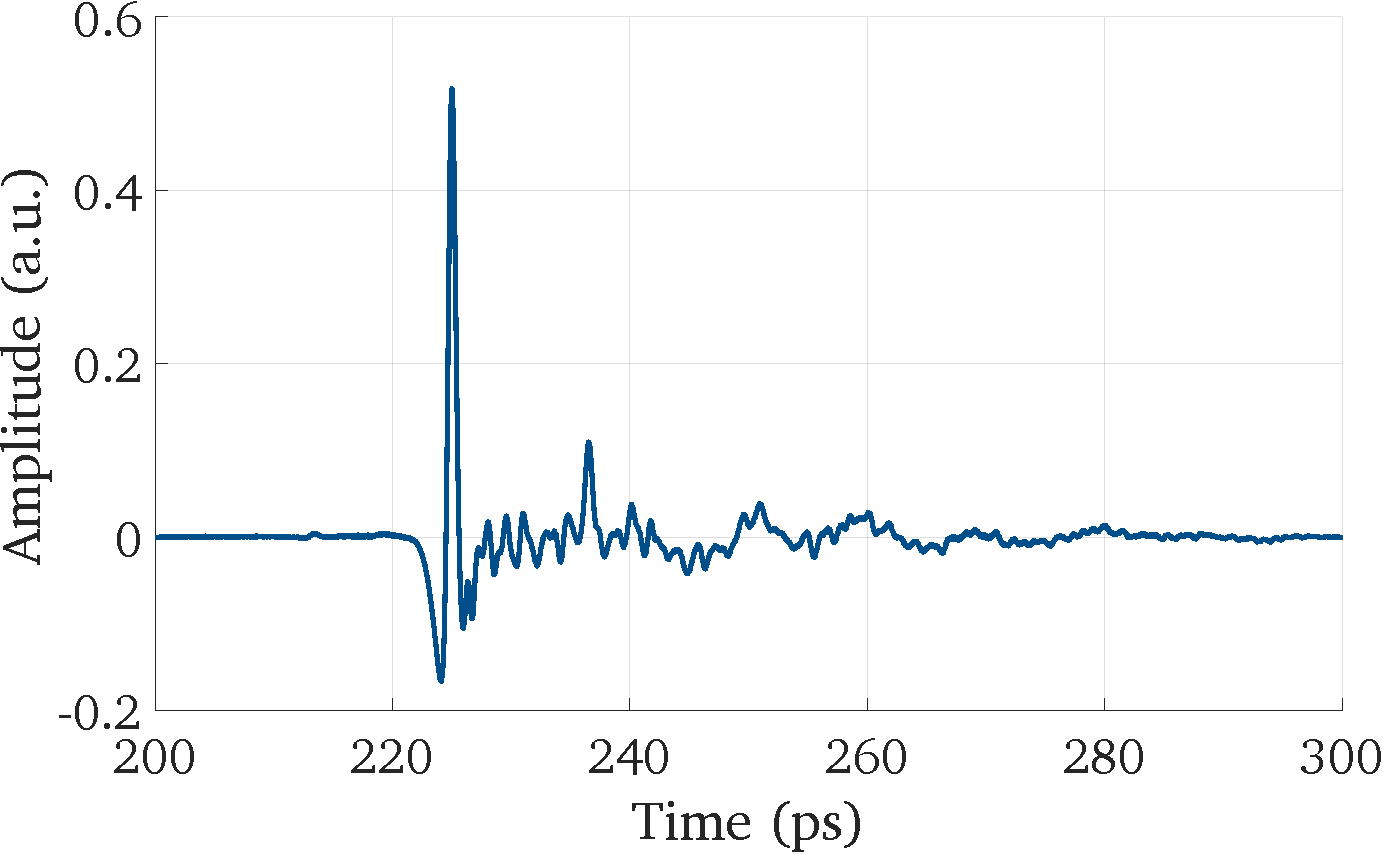
\includegraphics[width=0.6\linewidth]{figures/ringing_schem.pdf}
    \caption{A THz pulse is observed, followed by distinct time-domain harmonics appearing after the main pulse. The first noticeable peak resulting from standing waves occurs at approx. \num{240} \si{\pico \s}. Subsequent peaks appear every \num{10} \si{\pico \s}, resulting in an oscillation period $T \approx 20$ \si{\pico \s}. This corresponds to a resonance in the spectrum at $f \approx 50$ \si{\giga \hertz}, caused by standing waves in the antenna Structure.} 
    \label{fig:ringing}
\end{figure}